\begin{figure}
\centering
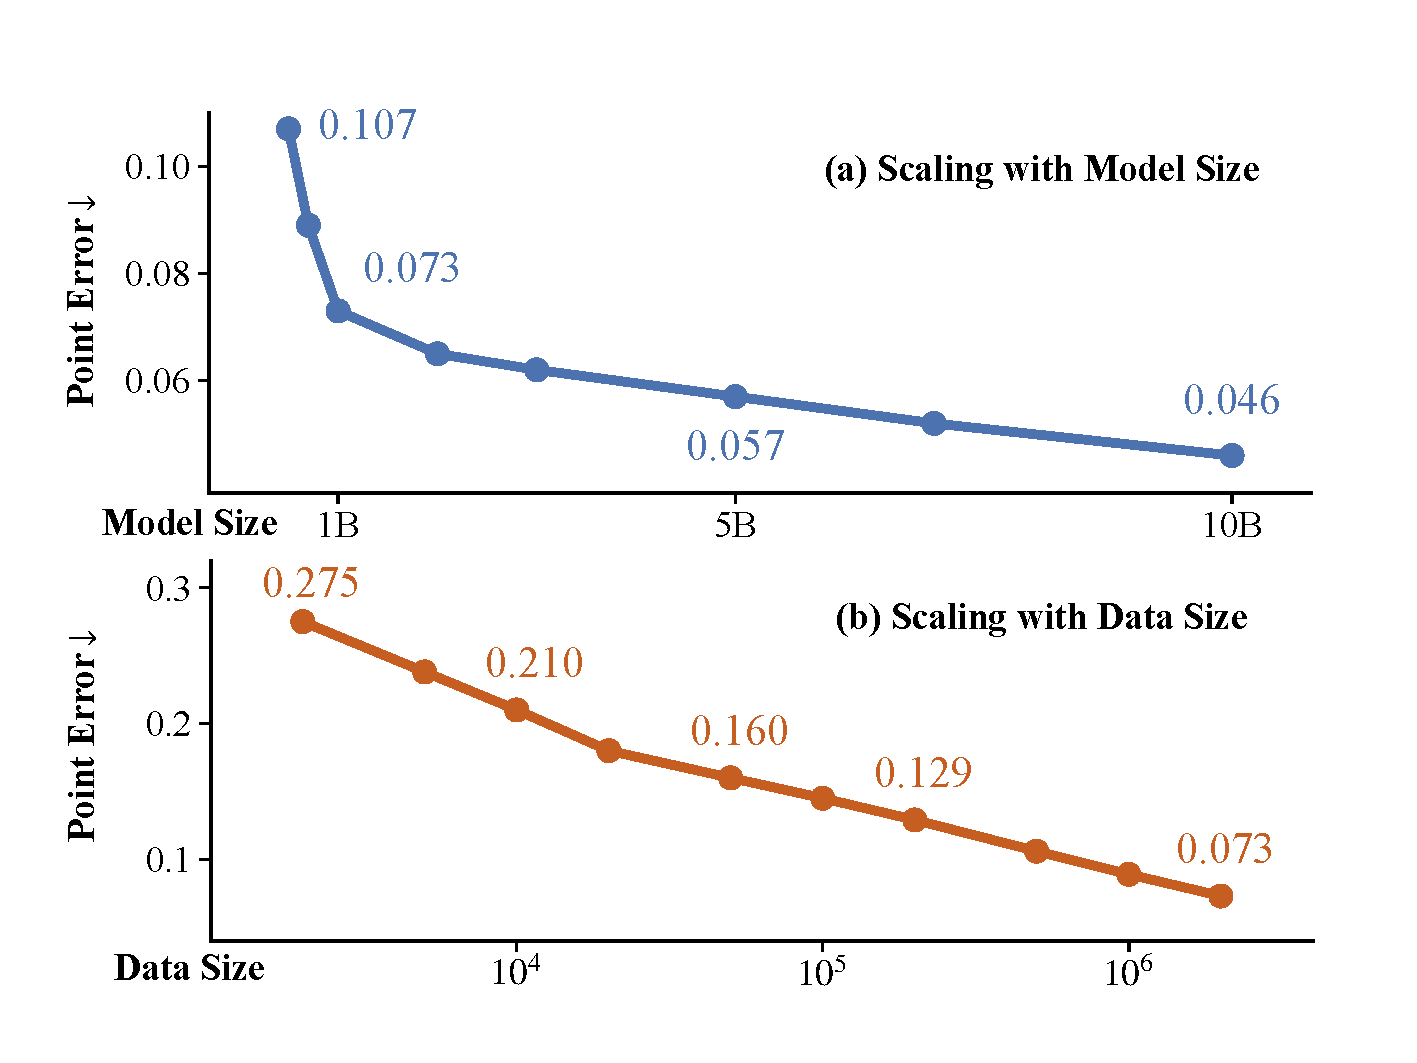
\includegraphics[width=0.95\linewidth]{figures/scale_v5_vector.pdf}
\caption{\textbf{Performance Gains from Data and Model Parameter Scaling.}
As model size increases from 0.2B to 10B parameters and data scale grows from 2K to 2M sequences, performance improves consistently, as measured by 3D point error (lower is better; note the different axis scales).
All models are trained on approximately the same number of tokens and evaluated by averaging over six datasets, with details provided in \cref{sec:benchmarking}.
}%
\label{fig:scale}
\vspace{-10pt}
\end{figure}


